% Author: Till Tantau
% Source: The PGF/TikZ manual
\documentclass[a4paper,11pt]{article}
\usepackage[utf8]{inputenc}
\usepackage{listings}
\usepackage{amsmath}    % need for subequations
\usepackage{graphicx}   % need for figures
\usepackage{verbatim}   % useful for program listings
\usepackage{color}      % use if color is used in text
%\usepackage{subfigure}  % use for side-by-side figures
\usepackage{hyperref}   % use for hypertext links, including those to external documents and URLs
\usepackage{url}
\usepackage{float}
\usepackage{todonotes}
\usepackage{tikz}
\usepackage{enumitem}
\usepackage{hyperref}
\usepackage{pdfpages}
\usepackage{caption}
\usepackage{epsfig}
\usepackage{subcaption}
\usepackage{listings}
\usepackage{color}
\usepackage{amsfonts}
\usepackage{latexsym}
\usepackage[T1]{fontenc} % use for allowing < and > in cleartext
\usepackage{fixltx2e}    % use for textsubscript
\usepackage[linesnumbered,boxed,ruled]{algorithm2e}
\usepackage{mathtools}
\DeclarePairedDelimiter{\ceil}{\lceil}{\rceil}
%\newcommand{\BigO}[1]{\ensuremath{\operatorname{O}\left(#1\right)}}
\newcommand{\BigO}[1]{\ensuremath{\mathop{}\mathopen{}\mathcal{O}\mathopen{}\left(#1\right)}}
\definecolor{mygreen}{rgb}{0,0.6,0}
\definecolor{mygray}{rgb}{0.5,0.5,0.5}
\definecolor{mymauve}{rgb}{0.58,0,0.82}
\lstset{ %
  backgroundcolor=\color{white},   % choose the background color; you must add \usepackage{color} or \usepackage{xcolor}
  basicstyle=\footnotesize,        % the size of the fonts that are used for the code
  breakatwhitespace=false,         % sets if automatic breaks should only happen at whitespace
  breaklines=true,                 % sets automatic line breaking
  captionpos=b,                    % sets the caption-position to bottom
  commentstyle=\color{mygreen},    % comment style
  deletekeywords={...},            % if you want to delete keywords from the given language
  escapeinside={\%*}{*)},          % if you want to add LaTeX within your code
  extendedchars=true,              % lets you use non-ASCII characters; for 8-bits encodings only, does not work with UTF-8
  %frame=single,                    % adds a frame around the code
  keepspaces=true,                 % keeps spaces in text, useful for keeping indentation of code (possibly needs columns=flexible)
  keywordstyle=\color{blue},       % keyword style
  language=Octave,                 % the language of the code
  morekeywords={*,...},            % if you want to add more keywords to the set
  numbers=left,                    % where to put the line-numbers; possible values are (none, left, right)
  numbersep=5pt,                   % how far the line-numbers are from the code
  numberstyle=\tiny\color{mygray}, % the style that is used for the line-numbers
  rulecolor=\color{black},         % if not set, the frame-color may be changed on line-breaks within not-black text (e.g. comments (green here))
  showspaces=false,                % show spaces everywhere adding particular underscores; it overrides 'showstringspaces'
  showstringspaces=false,          % underline spaces within strings only
  showtabs=false,                  % show tabs within strings adding particular underscores
  stepnumber=2,                    % the step between two line-numbers. If it's 1, each line will be numbered
  stringstyle=\color{mymauve},     % string literal style
  tabsize=2,                       % sets default tabsize to 2 spaces
  %title=\lstname                   % show the filename of files included with \lstinputlisting; also try caption instead of title
}

\bibliographystyle{plain}
\begin{document}
\graphicspath{ {./images/} }
\date{May 21st 2014}
\title{Mining build orders in\\StarCraft 2: Heart of the Swarm}

\author{Andrea Catalini\\
\texttt{acat@itu.dk}
\and Michał Królikowski\\
\texttt{mikrl@itu.dk}
\and Rick Marker\\
\texttt{rdam@itu.dk}}

\clearpage\maketitle
\thispagestyle{empty}
\setcounter{page}{1}
\begin{abstract}
This report concerns analysis of the real time strategy game StarCraft 2. In the report a possible connection between a players sequence of actions and whether he will win or not, is studied. Extending on this question a connection between a players sequence of actions and the league in which he plays, is also being studied. 
For the first question, the C4.5 tree algorithm is used. For the second question, the k-means clustering algorithm is applied, and  an evaluation is performed, to see if the clusters produced represent the leagues.
The results of the experiment indicate, that if only the order in which actions are taken it is not possible to predict a winner with high accuracy, nor does it serve to predict a players league.
\end{abstract}

%\newpage
%\setcounter{page}{1}

\section{Introduction}
In this paper we will look at the real time strategy game “StarCraft 2” by Blizzard Entertainment. 
In StarCraft 2, the player commands an army of one of 3 races: Protoss, Terran or Zerg. The game features “1 vs 1” mode, in which two players compete against each other, and a teamplay mode, with more armies involved.
To be able to balance the game, a league system is used. As the players skills increase, they win more matches and thereby advance to better leagues, to be matched against equally skilled players.
Having reached 3.000.000 registered players, the game holds a steady position among the worlds most popular e-sports. That makes it an interesting domain to study.
Specifically, we will focus on the action order of StarCraft 2 games. The action order is the chronological order in which a player builds units and uses abilities throughout a game. Based on this data, we will answer the following questions:
\begin{enumerate}
%\item Is it possible to predict what race this player played against? \label{q:opponent}
\item Is it possible to predict if the player will win?\label{q:win}
\item Does clustering the action order of various players, clearly separate the leagues?\label{q:league}
\end{enumerate}

To answer those questions, we used WEKA - an open source data mining environment, implementing various mining algorithms, along with preprocessing and visualisation methods. We also generated graphs depicting the distribution of action order paths taken by the players.
We explored question [\ref{q:win}] using the C4.5 tree algorithm. Apart from the answer to the stated question, we were also interested in seeing the first branchings of the generated trees, as the features that they represent are the best predictors about who could win. 
For the question [\ref{q:league}] we have used the k-means algorithm to check if the action order was related to the league index. It was interesting to see if the action order alone was characteristic enough to distinguish good players from bad ones, assuming good players were in better leagues.

\subsection{Data set}
The data used was obtained by crawling a popular archive \url{Gamereplays.org} for data files.
The files obtained were natively in a 'sc2replay' format, used by the StarCraft 2 engine to record and replay games. Due to differences in the structure of the replays generated by the existence of different patches of the game, we used only the files from the Heart of the Swarm expansion pack. This gave us 462 replay files. The replay files included various data about the games, but we were only interested in the following features: the outcome of the game, the player races, the player leagues, each player’s build- and ability order.
We note, that even though action timestamps were available in the files, the purpose of this report was to answer our questions based only on the order of actions.

\section{Preprocessing}
\label{sec:preprocessing}
We started by reformatting the obtained data sets, defining a single players build order as a tuple.
In effect this meant breaking ties between the players and their opponents, but as the only information we needed about the opponents were the races, we added this information to the new player-tuples.
The data was then cleaned from noise generated by modded predefined games. Those are games in which the regular StarCraft 2 rules are altered. Games like those were filtered by removing the tuples where players performed actions that were considered invalid according to the regular games. We note that this may not have removed all the modded games, as multiple Starcraft 2 mods exist, and not all of them involve buildings. Furthermore, it is possible that some matches that involved the Zerg race may have been incorrectly filtered, as one of the units of the Zerg army has an ability to take control of an opposing unit. The ability is rarely used though, so we considered this a fair trade-off.

Afterwards, we limited the dimensions of the data. As each race is able to do about 70 different actions (depending on race), and 280 actions are performed on average per game, the initial space was too sparse with those dimensions. Hence the team decided to group the actions into categories, instead of considering each action individually. Eventually 7 categories were created: \textit{Structure for building fighters}, \textit{Structure to improve economy}, \textit{Defensive structure}, \textit{Worker}, \textit{Ground unit}, \textit{Advanced fighter unit}, \textit{Upgrade}.

The next necessary step was reducing the list of actions taken. Different approaches were tried. In the initial approaches, we grouped the actions into bins of five, then we extracted the most frequent one among them as the value of the bin. Unfortunately those results were unsatisfactory, so the team decided to group the actions according to the resource usage. 

Each bin of the actions represented a fraction of the total resources obtained and spent by the player throughout the game.
As multiple kinds of resources exist in StarCraft 2, we decided to assign weight to each of them, so that a straightforward comparison could be made. For this we asked a domain specialist about his best approximation of weights.
As only one person was consulted and no clear consensus are established on the subject, these weights introduced some bias into the experiment.
Furthermore a dynamic growth of the bins was introduced, as the early actions in the game are usually cheaper, but not less significant. Otherwise, the players that vastly develop their economy, would have too large bin sizes at the beginning of the game. The sizes of the bins were chosen by empirical approximation of fair splits for the bins.

\section{Predicting A Winner}
For predicting the winner we have chosen a decision tree algorithm. This would not only answer our question, but also provide insight into the most relevant features for the winner prediction. More specifically, we have chosen WEKA’s J48 implementation of the C4.5 algorithm. It served our case better than ID3, because of its strength in processing attributes with large number of values.
C4.5 and ID3 classify as supervised learning algorithms - they need a training set with predictors, and with the resulting class to be able to work. Furthermore they are both eager in the way they process data from training sets, meaning they spend more time during training, but are faster at predicting.
They both also rely on Information Gain in order to decide on which attributes to split, Information Gain being a measure of the reduction in Information Entropy the split would generate. One difference between ID3 and C4.5 is that ID3 uses the Information Gain as it is, and C4.5 uses a normalized version. C4.5 also has other properties negligible in our case, i.e. C4.5 is able to handle numeric values and missing values.
Both algorithms work recursively by first looking at all the whole data set, and finding the feature which provides the most Information Gain. Once found, one branch for each value of the feature is created. At the next level, the chosen feature is disregarded, and the same approach is used for each branch. The algorithm stops if:

\begin{itemize}
\item all the elements in the subset belongs to the same class, in which case that node becomes a leaf
\item there are no remaining attributes for further partitioning
\item the subset have no examples left
\end{itemize}

In the first approaches, we have been using the data binned by actions. Then, we were able to answer correctly in 53\% cases. For a comparison, ZeroR, answers correctly 50.1\% of the time. Then, we switched to resource based binning, as explained in section \ref{sec:preprocessing}. We have also decided to split the data according to player armys race, instead of analyzing all the games at once. By tuning the confidence factor, the minimum number of objects per leaf and the degree of pruning, we managed to get just below 60\% correct classifications. It did however require individual settings for each race, which suggests, that no clear relation exist, and it depends too much on the parameters.
Figure \ref{fig:win:zerg} shows the resulting trees for Zerg. To our surprise the resulting trees does not gain much accuracy by adding more layers. For Zerg this is evident as the most pruned tree is correct 56\% of the time, and the less pruned tree is correct 54\% of the time. Were the values for each feature chosen at random, the resulting trees would look similar.
The trees for Protoss and Terran, which can be found in the Appendix, look very similar to Figure \ref{fig:win:zerg}. 
\begin{figure}[H]
\centering
\begin{subfigure}{.4\textwidth}
  \centering
  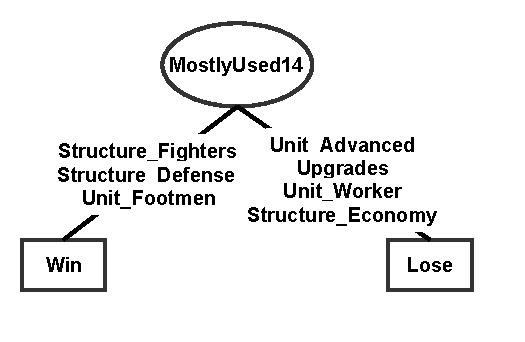
\includegraphics[width=.95\linewidth]{tree_zerg_pruned}
\end{subfigure}%
\begin{subfigure}{.4\textwidth}
  \centering
  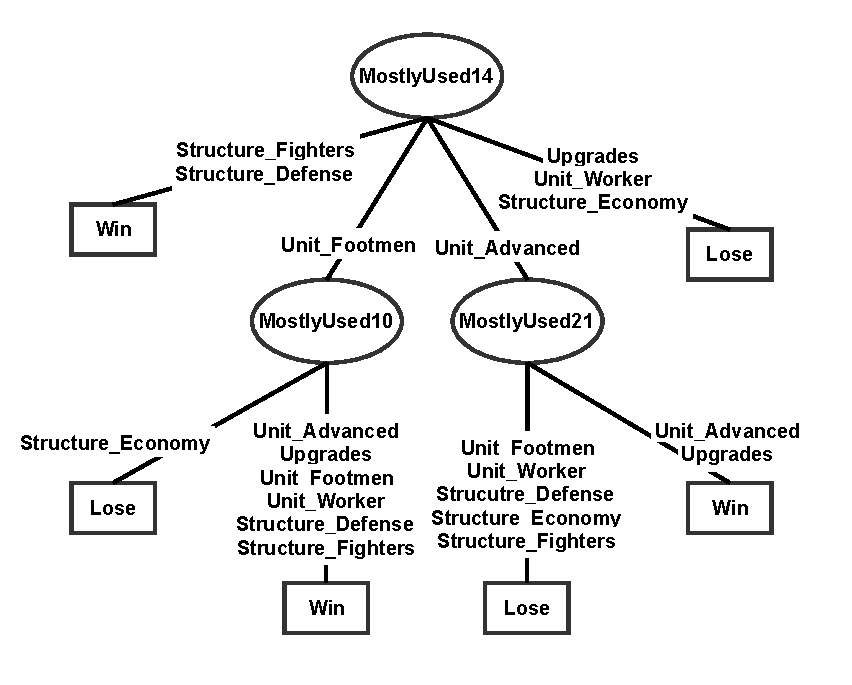
\includegraphics[width=.95\linewidth]{tree_zerg_unpruned}
\end{subfigure}
\caption{The pruned and unpruned decision tree of Zerg. Pruned version has correctly 56\% of time times and the unpruned 54\%}
\label{fig:win:zerg}
\end{figure}

In an additional test, the 3 race datasets were further divided according to the race of the opponent. The results showed to be very similar to when the opponent race was not taken into consideration. Because of that, we consider that the actions that the players took are not related to the race of their opponents. Hence the team decided to keep the penultimate results for greater readability and because splitting the dataset so much left us with very small subsets, which was considered a threat to its validity.
Our conclusion is that although we got up to 60\% correct classifications, only a very weak connection between the action order and game outcome exist. Furthermore we note that splitting the data set based on the players race, made our data sets much smaller. For our results to be considered robust the experiment should be repeated with a larger data set.

\section{Clustering the data}
The team tried to see if it was possible to discover the league the player belongs to, based on the action order. For this, we have used cluster analysis. This kind of analysis tries to find similarities between data. It groups the tuples with high affinity together, trying to keep the concept of high intra-class similarity and low inter-class similarity. It is an unsupervised learning method, which means that the training set that it obtains has no class labels - they are unknown. This method is usually used when looking for hidden structures in data.

The algorithm uses an initial k attribute that corresponds to the numbers of clusters to be generated. Its first step is division of the dataset in k nonempty subsets. K-means also has another input - the seed, which used for obtaining the centroids - the “middle” values of each cluster. As the initial subsets are created and their centers are defined, the algorithm iterates over the tuples, reassigning each object to the cluster with the nearest centroid. The distance between a value and a centroid is based on the previously mentioned distance metric. This process iterates, until the clusters stabilize.

As all our features were nominal, Hamming distance\footnote{If two values are the same the distance is 0, if they are not the same the distance is 1} was used as distance metric.
Just like in the previous section, the tests were initially conducted on the data of all the races merged together binned by actions. We have later divided the data and binned it by the resource usage.
For every format of the dataset, the same logic about the number of clusters was applied. Initially, the k was defined as the amount of leagues that we had in our data - 8. This seemed the most logical choice to start with, however the result was not satisfactory, as players of different leagues were spread among all the clusters as shown in Figure \ref{fig:cluster-8}.
\begin{figure}[H]
\centering
  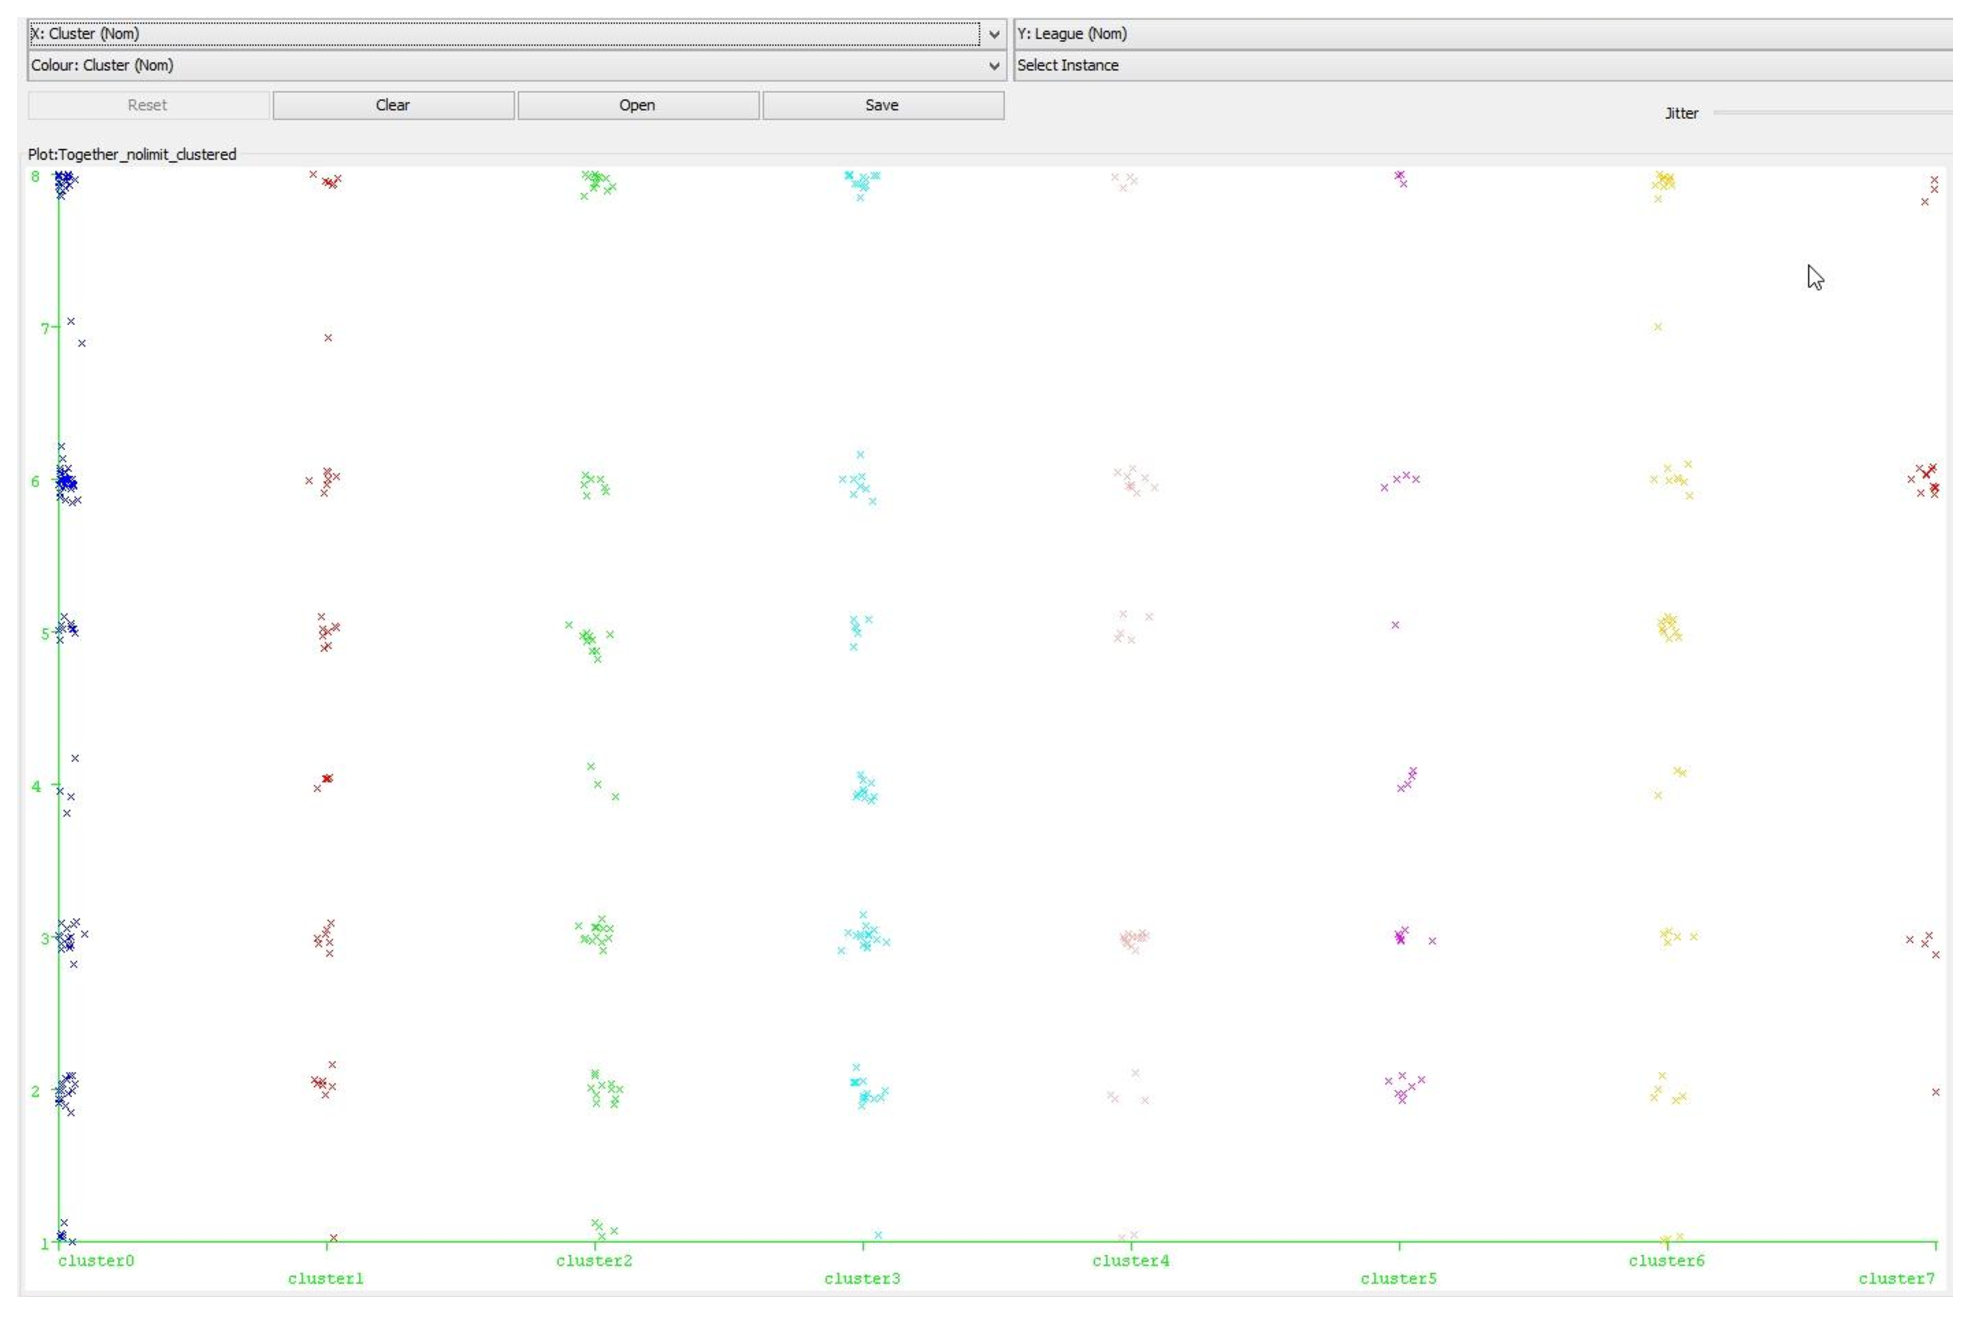
\includegraphics[width=.95\linewidth]{cluster-8}
\caption{Clustering of data. Clusters are on the x-axis and leagues are on the y-axis. Ideally each cluster should only contain data from one league.}
\label{fig:cluster-8}
\end{figure}

Then, since some of the leagues were much less less represented, the team decided to set k to the number of the biggest leagues - 5. Unfortunately the results was comparable to when 8 clusters were used.
The last test was conducted with an even smaller number, k = 3 and again the results were not different. The figures for the additional experiments can be found in the Appendix.

In all the tests the seed value was iterated upon 4 or 5 times with very far and random values. We wanted to see if different initial points for the k centroids could make a difference, but unfortunately it did not have any positive impact on the result.

With those results, we arrived at the conclusion that players cannot be classified into leagues, by simply checking their action order. More data is needed to be able to categorize by league.

\section{Additional validation - data visualization}
As an additional tool for our result validation, we created a tool for charting the distribution of players' actions throughout their games, and how it correlated to whether they would win and to their league.
The obtained charts confirmed our results. Very few factors stood out from the overall distribution in the graphs that depicts the outcome of the game, as seen in figure \ref{fig:sequence_win_zerg}, and no factors held any significance on the charts representing the league rankings, as seen in figure \ref{fig:sequence_league}. 
\begin{figure}[H]
\centering
  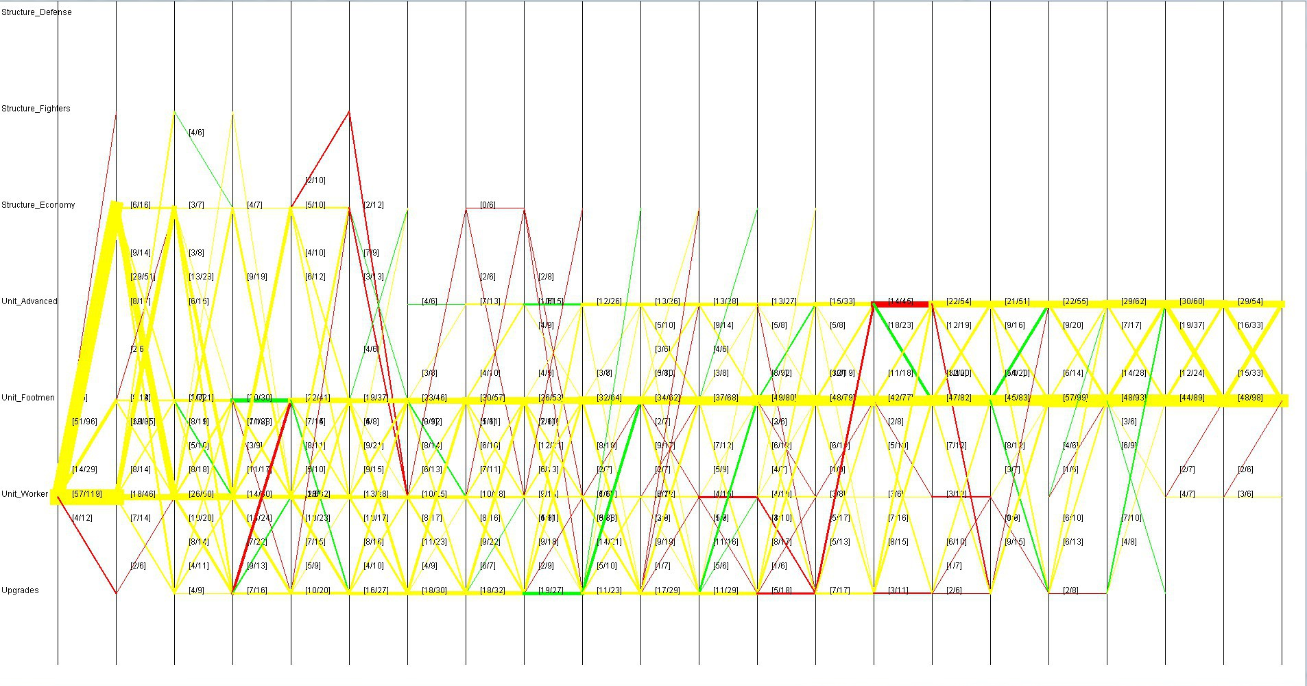
\includegraphics[width=.9\linewidth]{sequence_win_zerg}
\caption{Chart of the actions taken by Zerg players. Thickness represents frequency. y-axis is action, x-axis is time line. Color represents outcome. Green means mostly wins, red mostly loses, and yellow represents that wins and loses are evenly present}
\label{fig:sequence_win_zerg}
\end{figure}

\begin{figure}[H]
\centering
  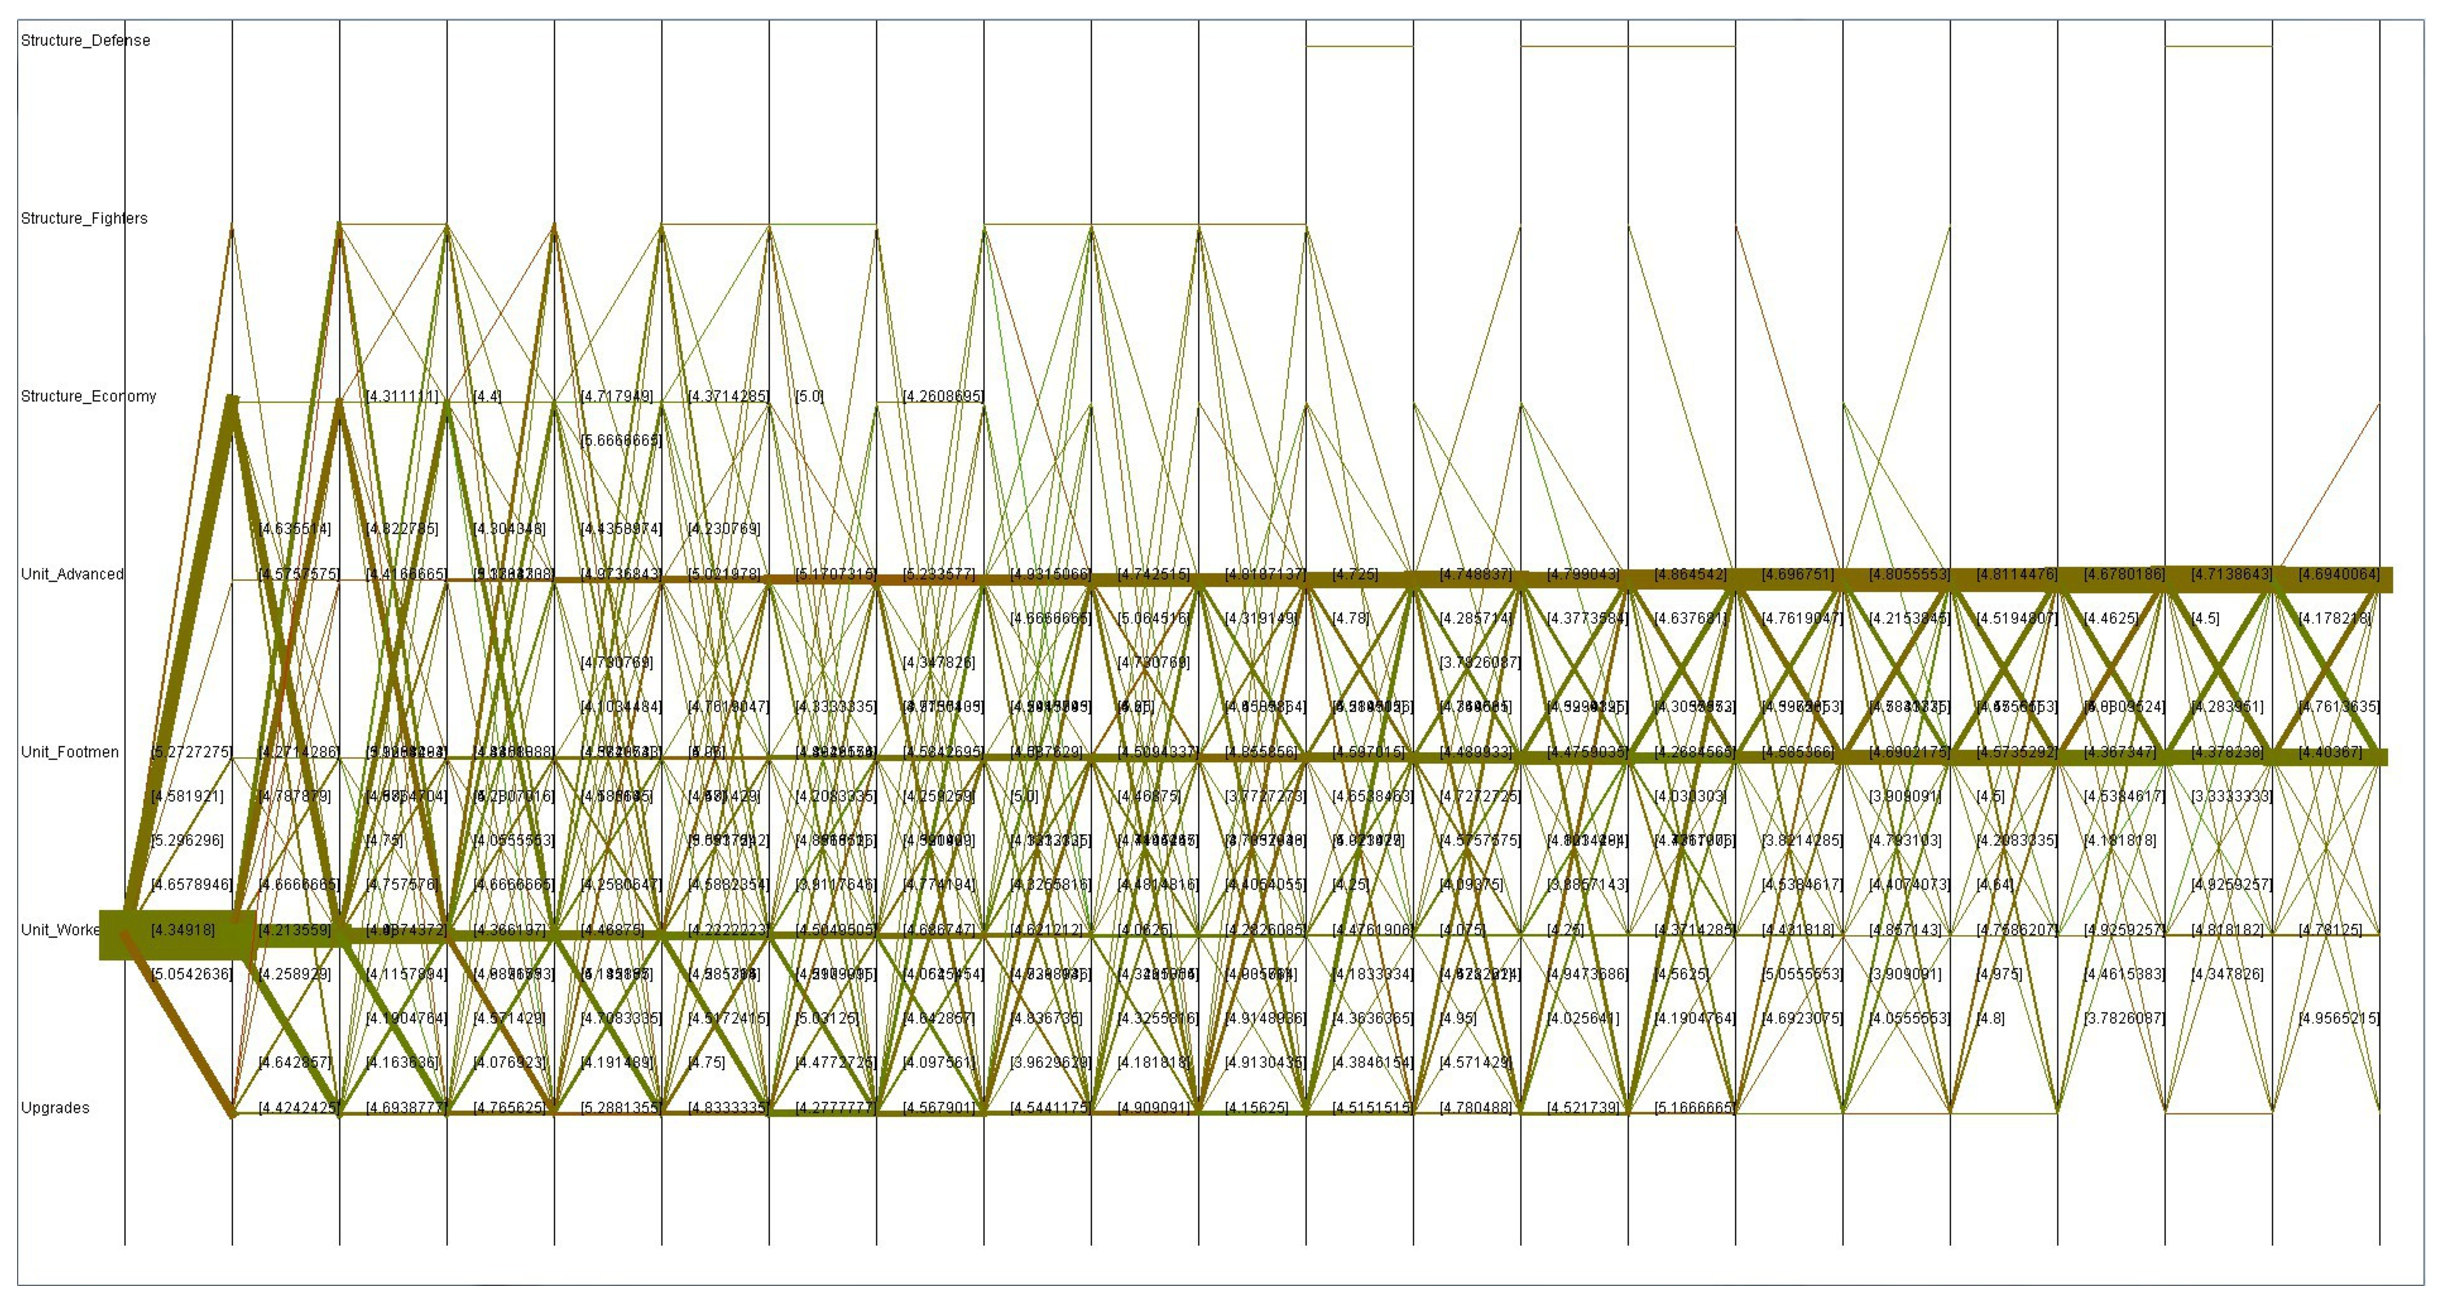
\includegraphics[width=.9\linewidth]{sequence_league}
\caption{Chart of the actions taken by Zerg players. Thickness represents frequency. y-axis is action, x-axis is time line. Colors is average league, green being league 1, and red league 8.}
\label{fig:sequence_league}
\end{figure}

\section{Discussion}
Our experiments prove that there is no strong correlation between the action order, the outcome of the match and the league they are in. Though, we realize that many improvements could be done in order to make our conclusion more sound.
First of all, a bigger data set should be used. This is very feasible as new replay files are uploaded every day.
Secondly one of the preprocessing actions required assigning weights to resource types. As our domain specialist noted, the weights in a game are not static, but they change according to the maps, and even during a single match. Having a static, preset value for each resource type will not reflect their values correctly.
It is worth noting, that the team, despite having some experience with the game, could have explored the domain knowledge more vastly, and could have used more domain specialists for consultation and brainstorming. One of the spheres where the domain knowledge might have helped more, was the unit classification The team had a difficulty assigning less stereotypical unit types into defined classes, and agreeing on the class definitions, as every race had some characteristic traits the others lacked. For example, a Protoss army includes many advanced unit types, some of which are not precisely fighters, but rather back-line support units. As the other armies lacked such units, we have decided not to introduce such division and to assign the support units into the same class as the heavy fighters.
In the last point of the discussion, we would like to point out, that even if the results of our game outcome prediction are not significant, we succeeded in nearly 60\% cases. Therefore, some knowledge might be obtained by analyzing the trees we have generated. For example: Protoss players are less likely to win if they are still spending their resources on upgrades in the 80\% of the game, and the Zerg players are typically more likely to succeed if they vastly produce small fighters between 40th\% and 60\% of the game time.
Should one extend upon the work, we would advise to take another, additional factor into account. That could be resource management, or possibly the actual build times, and not just the sequence information.

\section{Conclusion}
Although the data set used is too small to be able to obtain the desired level of robustness in our conclusion, our study has uncovered the following:
Using C4.5 algorithm, is not possible to clearly tell who is going to win a game of StarCraft 2 based on the order of a players actions. The best result achieved by our team was 59\% success rate for one of the races, which is not, in our eyes, significant.
Furthermore we have shown, by using clustering, that the order in which players perform actions does not relate to the league of the player in any clear way.
It is our opinion that further study in the area would benefit by extending the problem to include the actual timestamps at which buildings were produced, and by using a larger data set. Exploration of the domain knowledge more, and using the guidance of professional players and domain experts would be also advised for future work.\footnote{Thanks to Mike Debus, for providing domain knowledge}

\newpage

%code in appendix
\section*{Appendix}
\appendix
\section{Win/Lose}
\subsection{Trees}
  \begin{figure}[H]
    \centering
    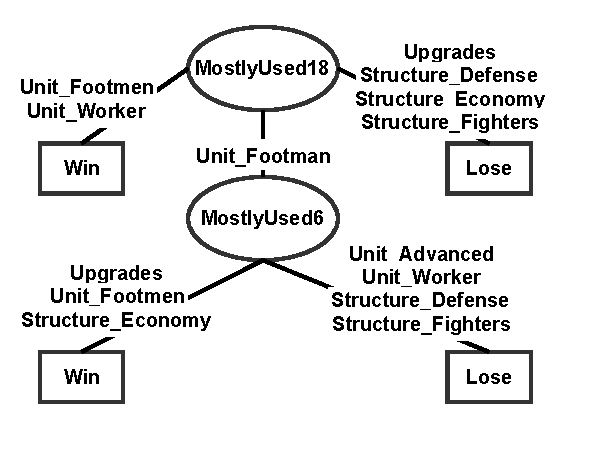
\includegraphics[width=.95\linewidth]{tree_protoss}
    \caption{The pruned decision tree for Protoss.}
  \end{figure}
  \begin{figure}[H]
    \centering
    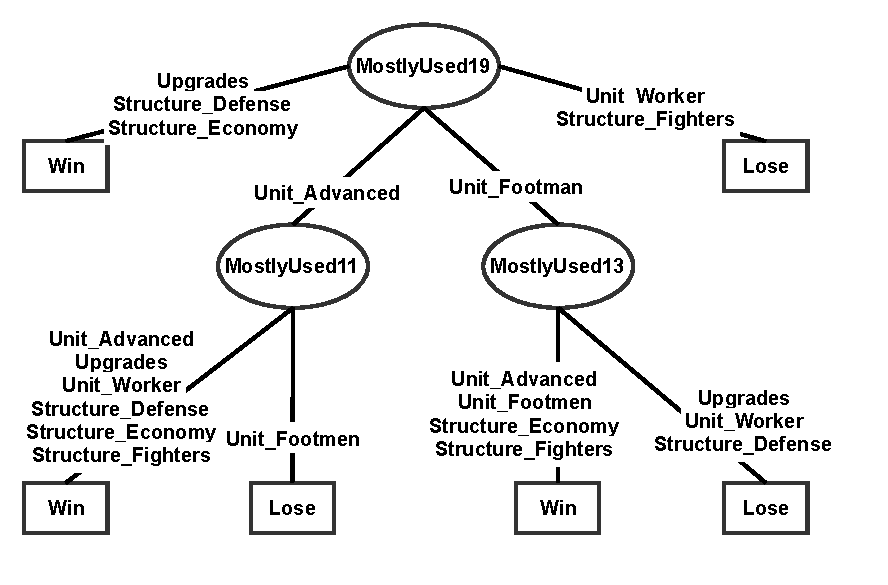
\includegraphics[width=.95\linewidth]{tree_terran}
    \caption{The pruned decision tree for Terran.}
  \end{figure}

\subsection{Validation}
  \begin{figure}[H]
    \centering
    \includegraphics[width=.95\linewidth]{winlose_all}
    \caption{Chart of the actions taken by all players. Thickness represents frequency. y-axis is action, x-axis is time line. Color represents outcome. Green means mostly wins, red mostly loses, and yellow represents that wins and loses are evenly present}
  \end{figure}
  \begin{figure}[H]
    \centering
    \includegraphics[width=.95\linewidth]{winlose_terran}
    \caption{Chart of the actions taken by Terran players. Thickness represents frequency. y-axis is action, x-axis is time line. Color represents outcome. Green means mostly wins, red mostly loses, and yellow represents that wins and loses are evenly present}
  \end{figure}
  \begin{figure}[H]
    \centering
    \includegraphics[width=.95\linewidth]{winlose_protoss}
    \caption{Chart of the actions taken by Protoss players. Thickness represents frequency. y-axis is action, x-axis is time line. Color represents outcome. Green means mostly wins, red mostly loses, and yellow represents that wins and loses are evenly present}
  \end{figure}

\section{Clustering}
\subsection{Clusters}
  \begin{figure}[H]
    \centering
    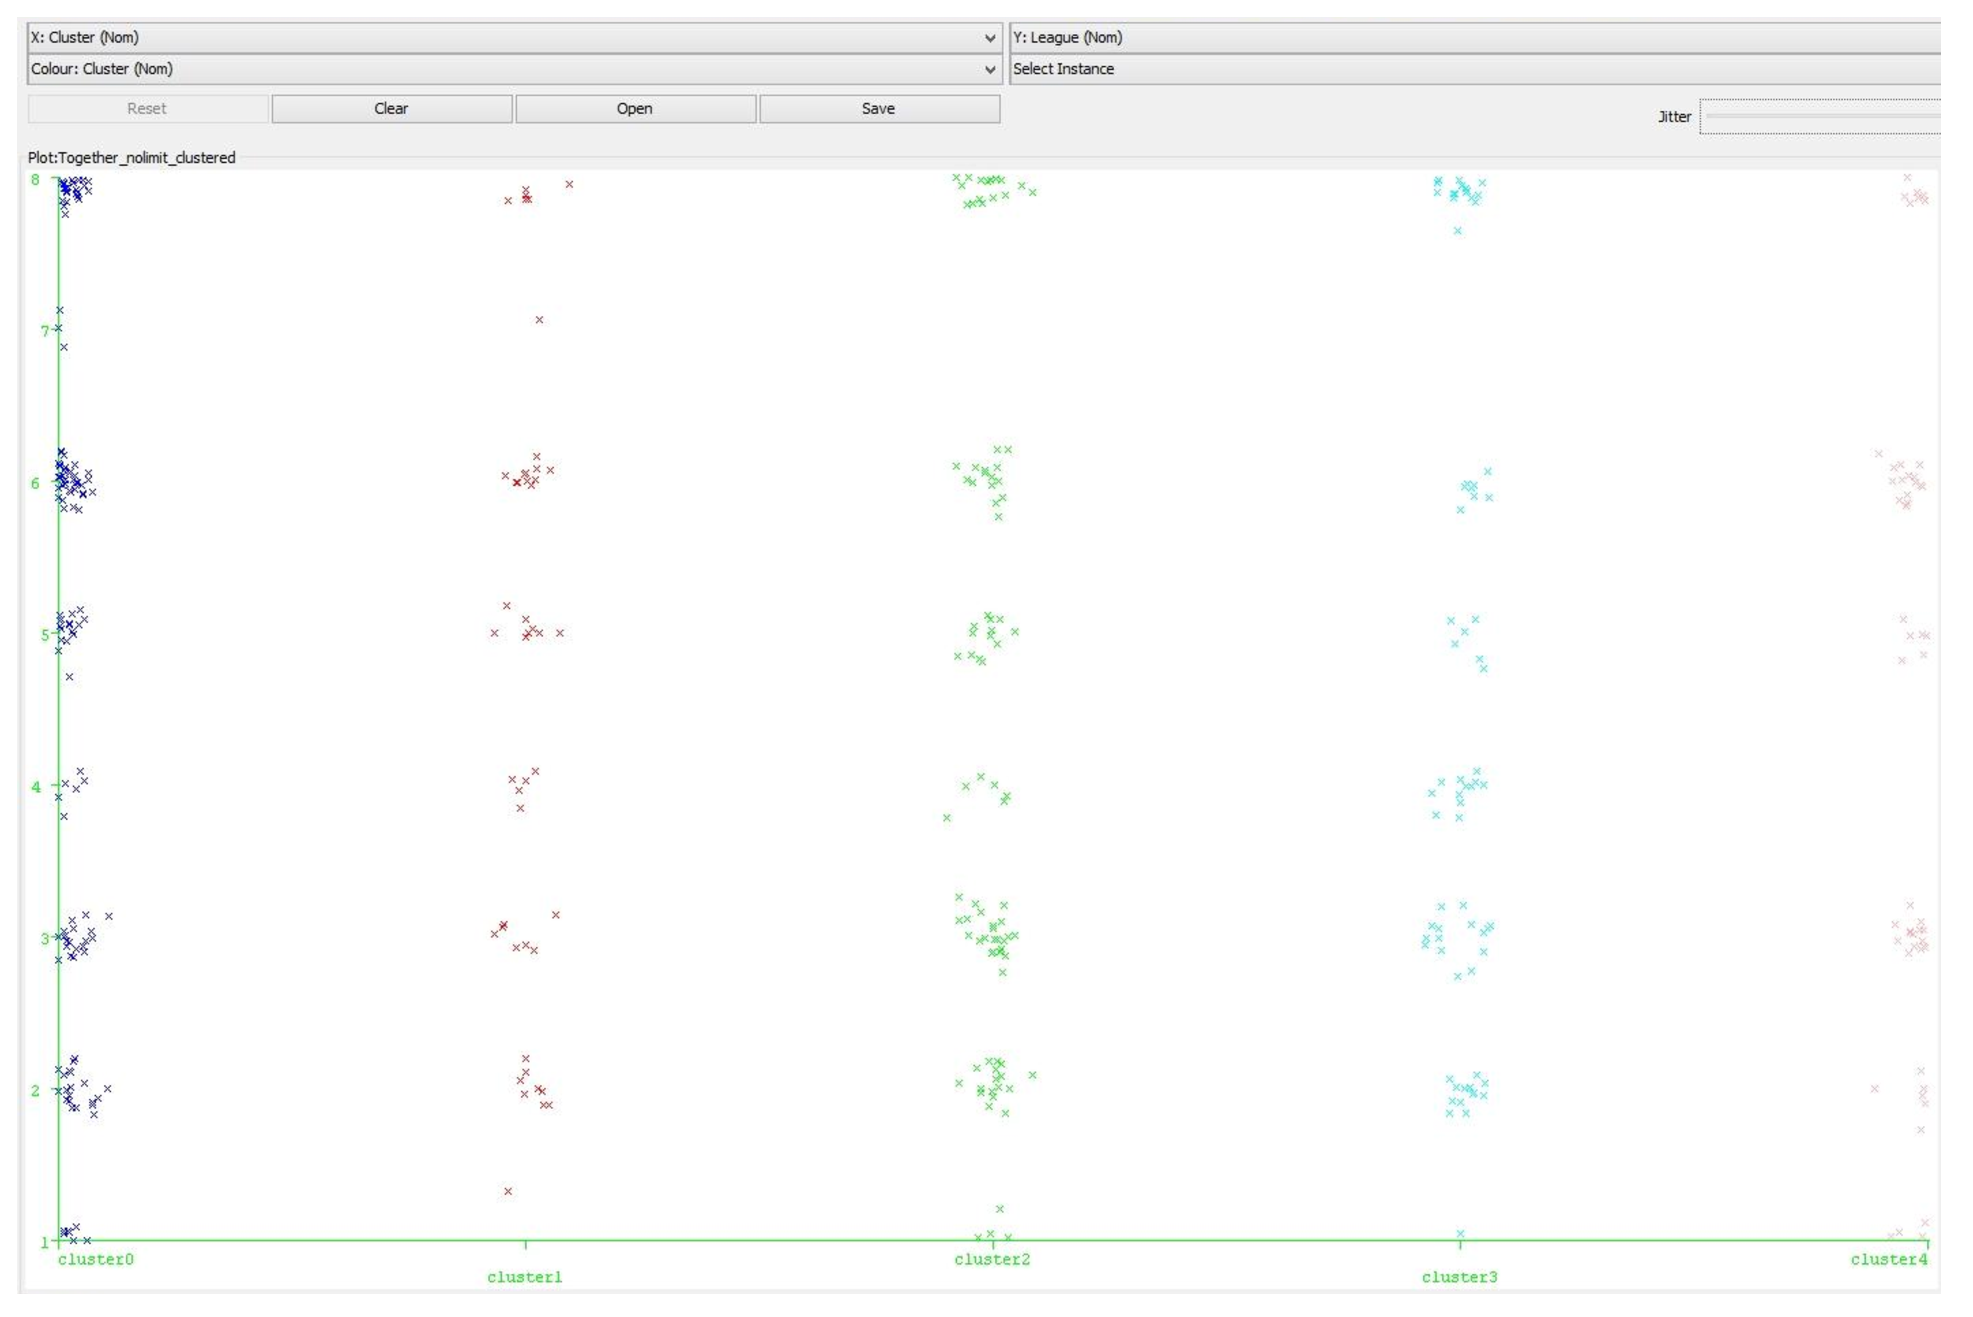
\includegraphics[width=.95\linewidth]{cluster-5}
    \caption{k-means with $k = 5$}
  \end{figure}
  \begin{figure}[H]
    \centering
    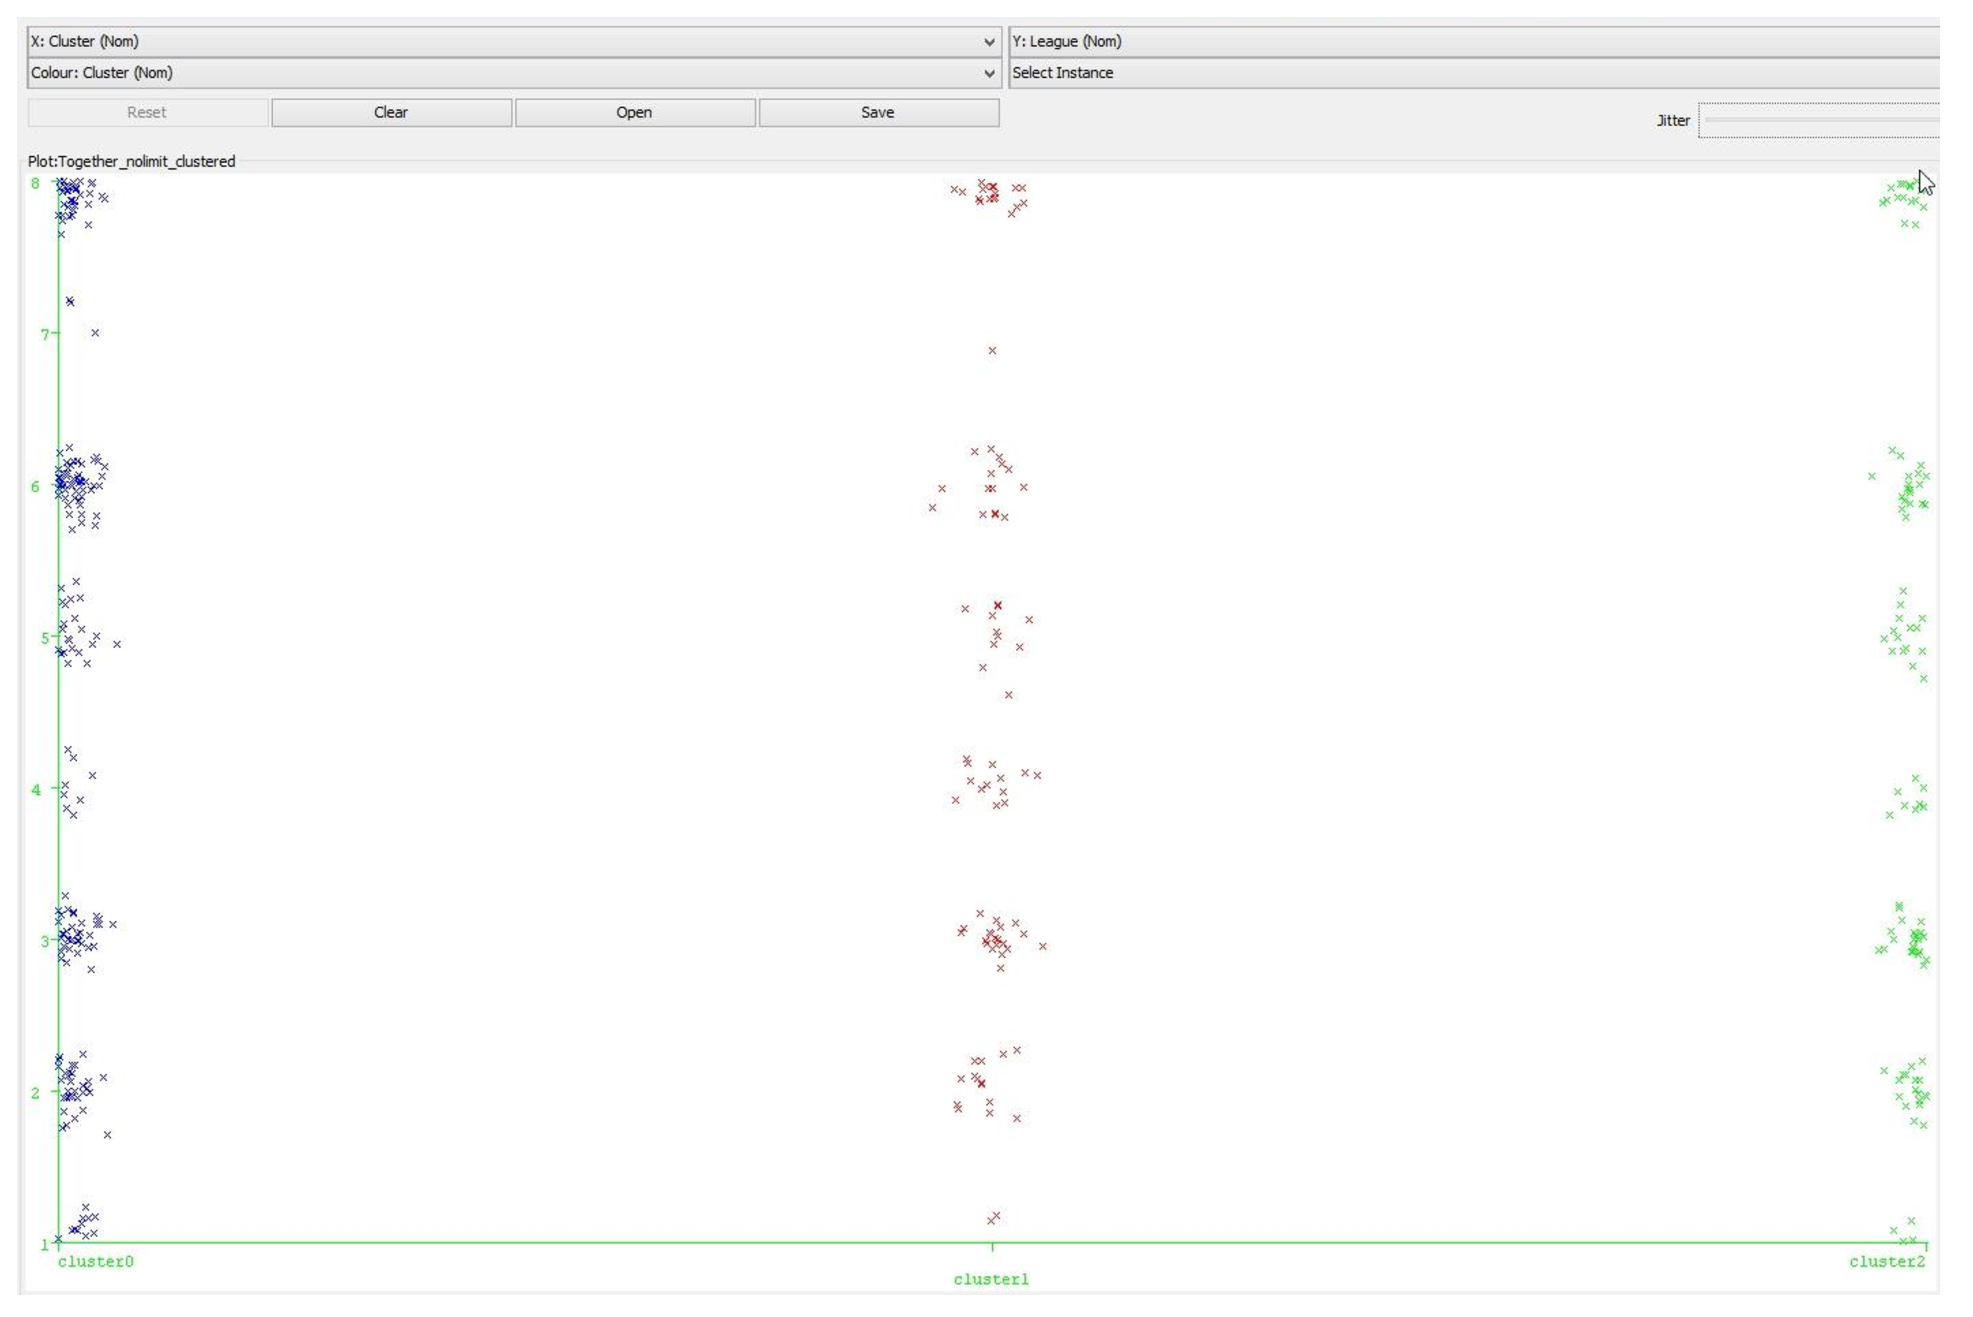
\includegraphics[width=.95\linewidth]{cluster-3}
    \caption{k-means with $k = 3$}
  \end{figure}
  \subsection{Validation}
  \begin{figure}[H]
    \centering
    \includegraphics[width=.95\linewidth]{league_all}
    \caption{Chart of the actions taken by all players. Thickness represents frequency. y-axis is action, x-axis is time line. Colors is average league, green being league 1, and red league 8.}
  \end{figure}
  \begin{figure}[H]
    \centering
    \includegraphics[width=.95\linewidth]{league_zerg}
    \caption{Chart of the actions taken by Zerg players. Thickness represents frequency. y-axis is action, x-axis is time line. Colors is average league, green being league 1, and red league 8.}
  \end{figure}
  \begin{figure}[H]
    \centering
    \includegraphics[width=.95\linewidth]{league_protoss}
    \caption{Chart of the actions taken by Protoss players. Thickness represents frequency. y-axis is action, x-axis is time line. Colors is average league, green being league 1, and red league 8.}
  \end{figure}
  \begin{figure}[H]
    \centering
    \includegraphics[width=.95\linewidth]{league_terran}
    \caption{Chart of the actions taken by Terran players. Thickness represents frequency. y-axis is action, x-axis is time line. Colors is average league, green being league 1, and red league 8.}
  \end{figure}

%\lstinputlisting[language=Python]{../src/dsbf.py}


\end{document}
